
\begin{figure}[H]
    \centering
    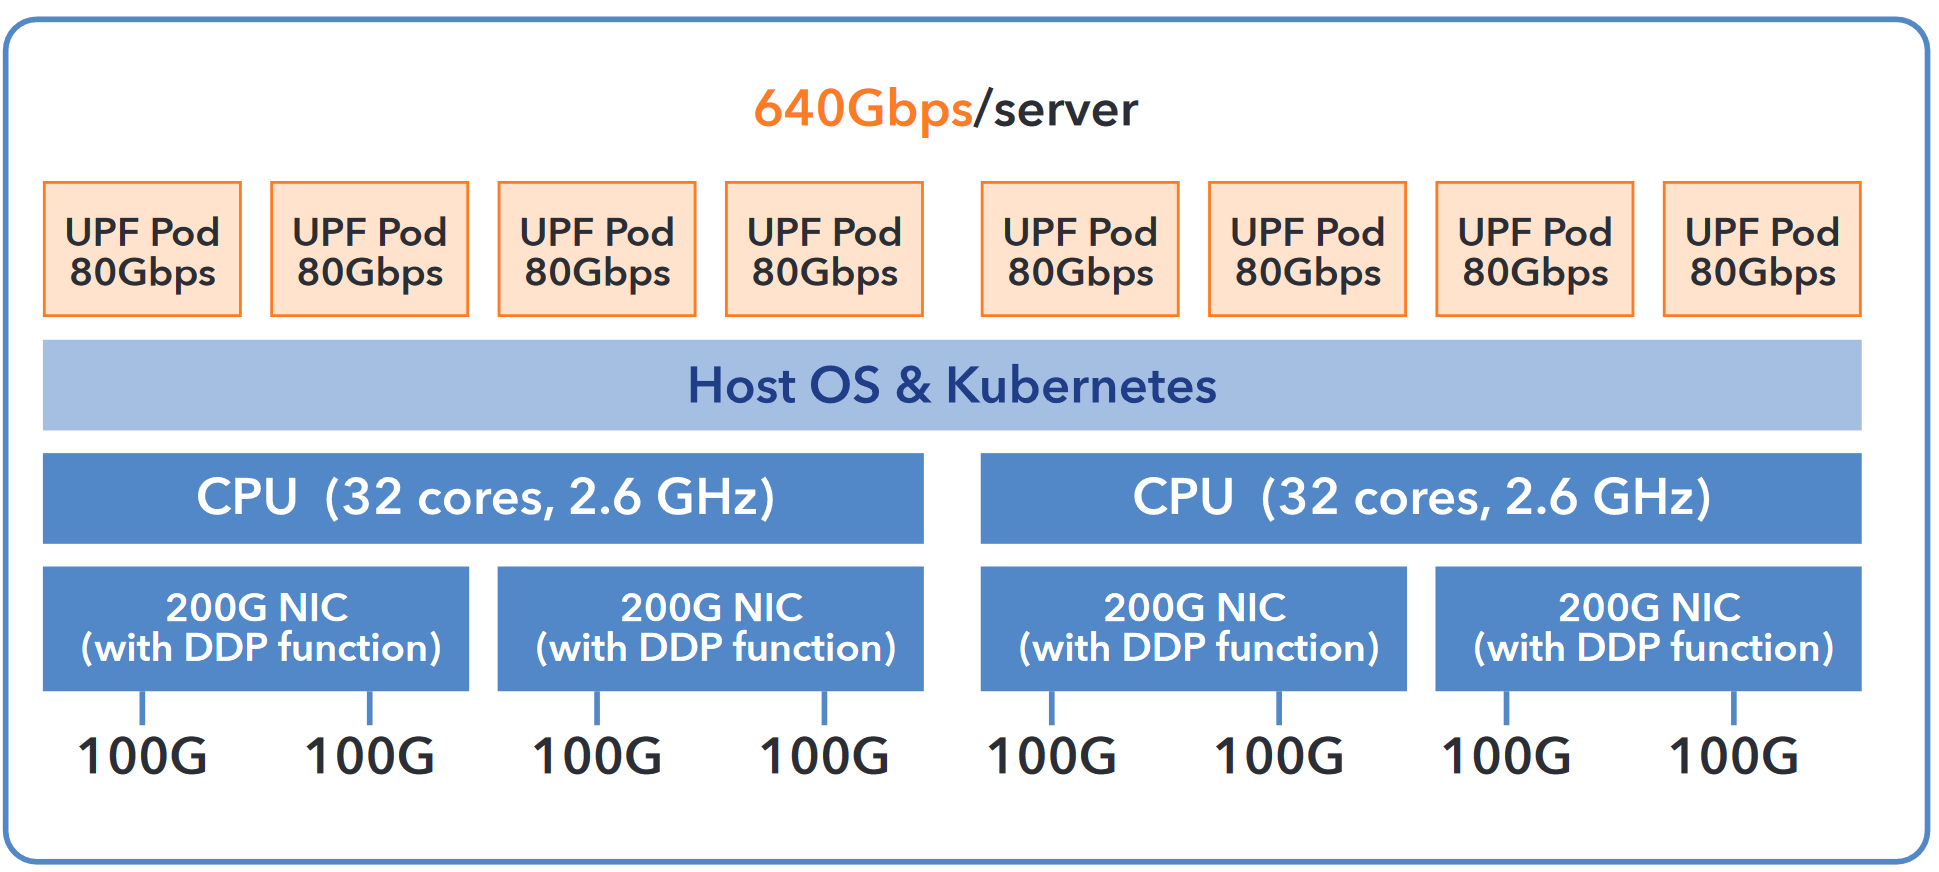
\includegraphics[width=0.6\textwidth]{resources/images/640_nec_upf_system.PNG}
    \caption{NEC's containerized UPF software (8 pods per server) on a platform configured with Linux and Kubernetes \cite{nec_upf_whitepaper}}
    \label{fig:sota:640_nec_upf_system}
\end{figure}

\begin{figure}[H]
    \centering
    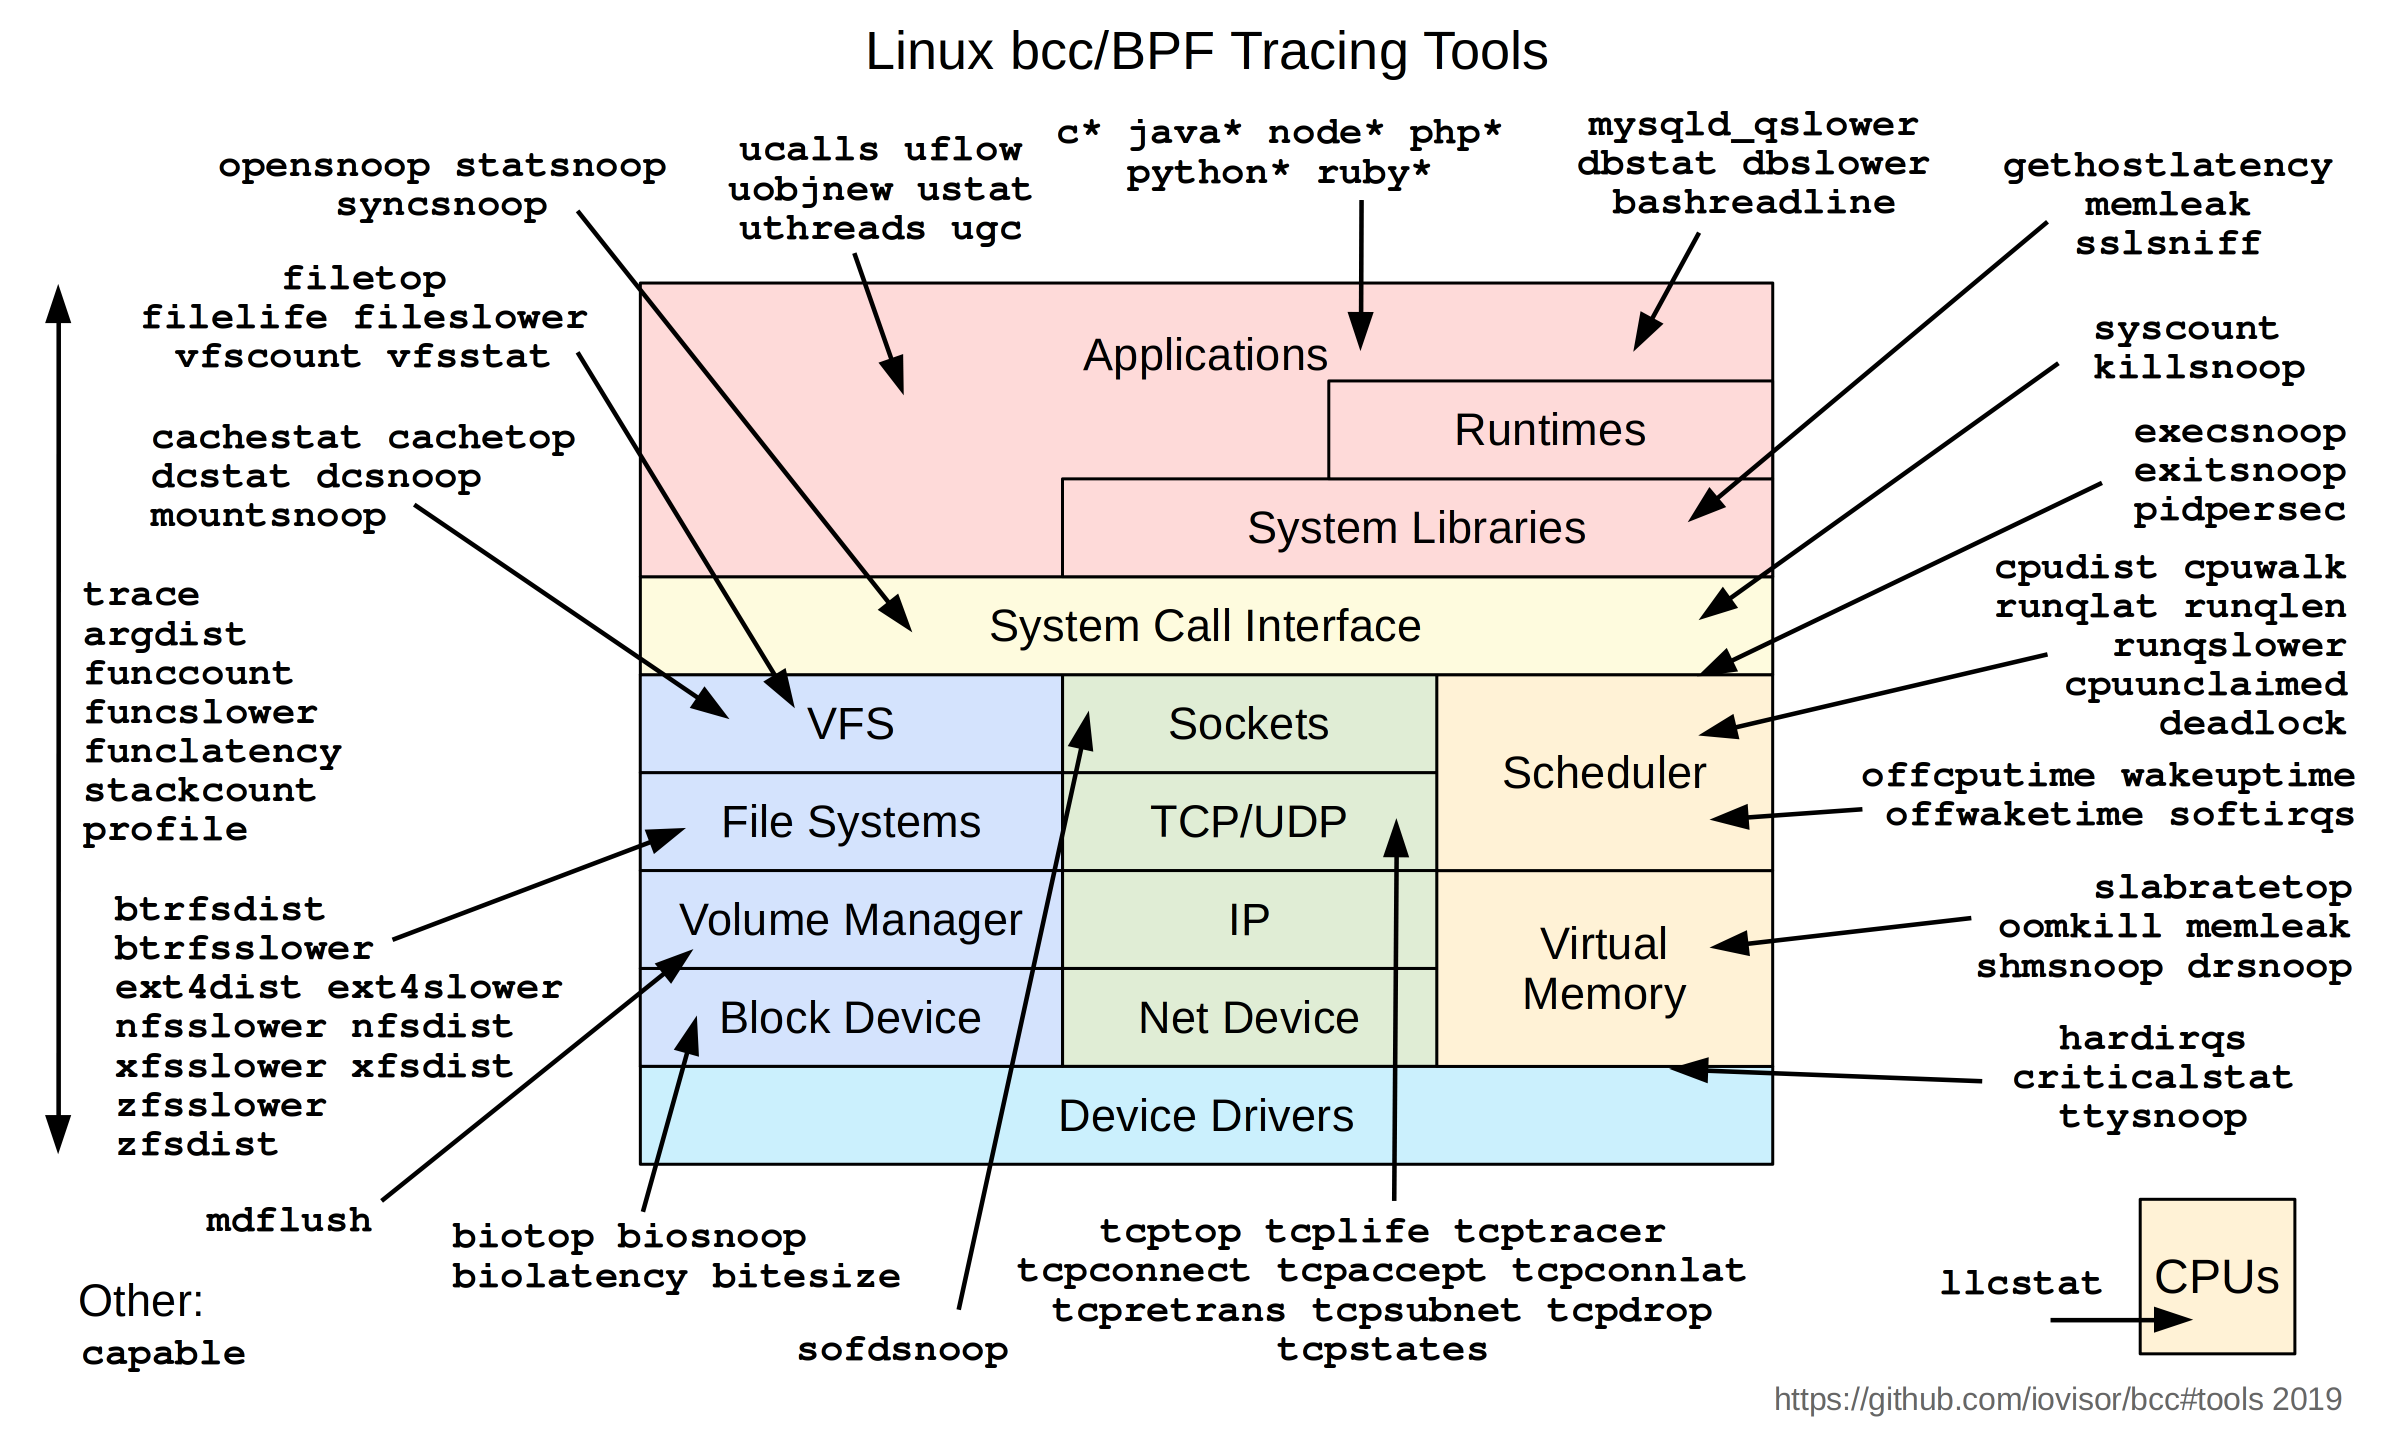
\includegraphics[width=1.0\textwidth]{resources/images/bcc_tracing_tools_2019.png}
    \caption{A wide range of Linux eBPF-based tracing tools \cite{iovisor_page}.}\label{fig:sota:tracing_tools_linux}
\end{figure}

\begin{figure}[H]
	\centering
	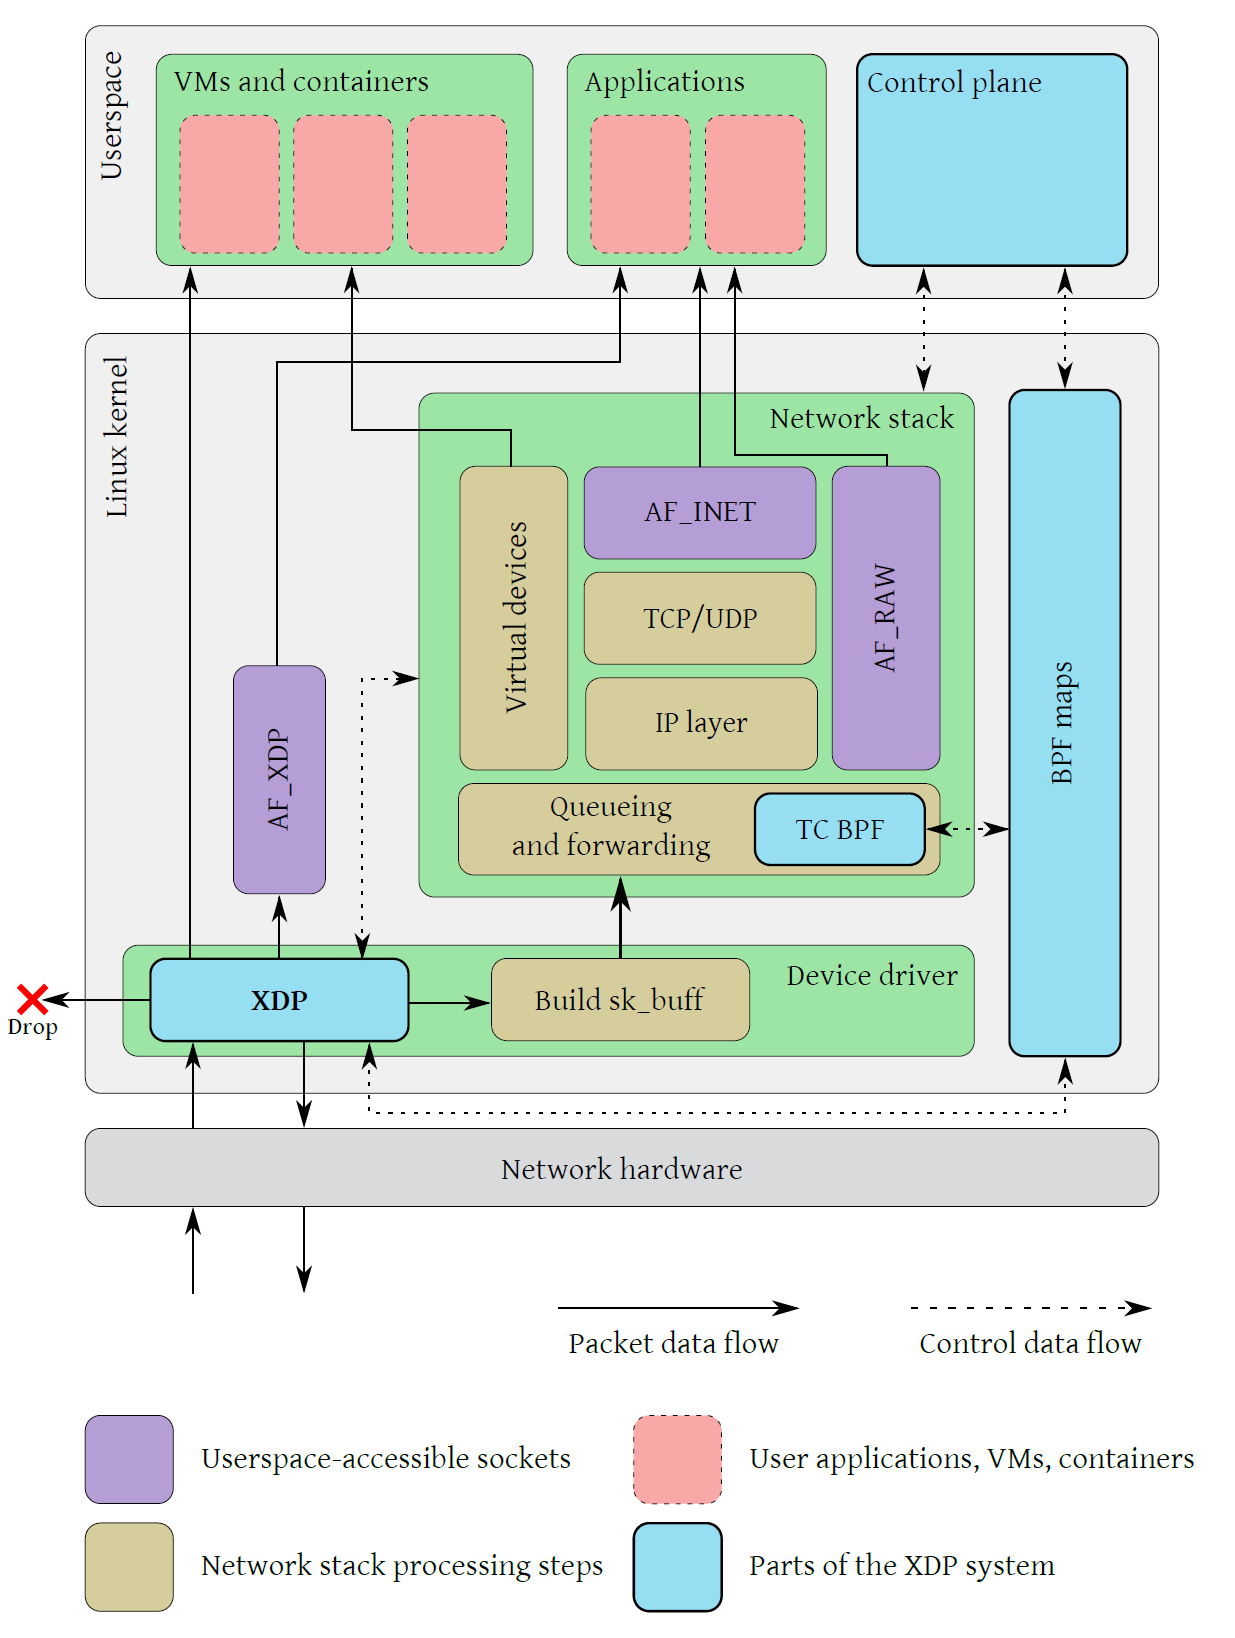
\includegraphics[width=1.0\textwidth]{XDP_integration_with_the_Linux_network_stack.PNG}
	\caption{XDP’s integration with the Linux network stack \cite{hoiland_jorgensen_express_2018}. The XDP program is activated whenever a packet enter the driver's buffer, where it will be examined. The XDP program makes the decision if the packet should follow its normal path in the network stack, or be discarded/forwarded/delivered to XDP user space program.}\label{fig:sota:xdp_architecture}
\end{figure}

\begin{figure}[H]
	\centering
	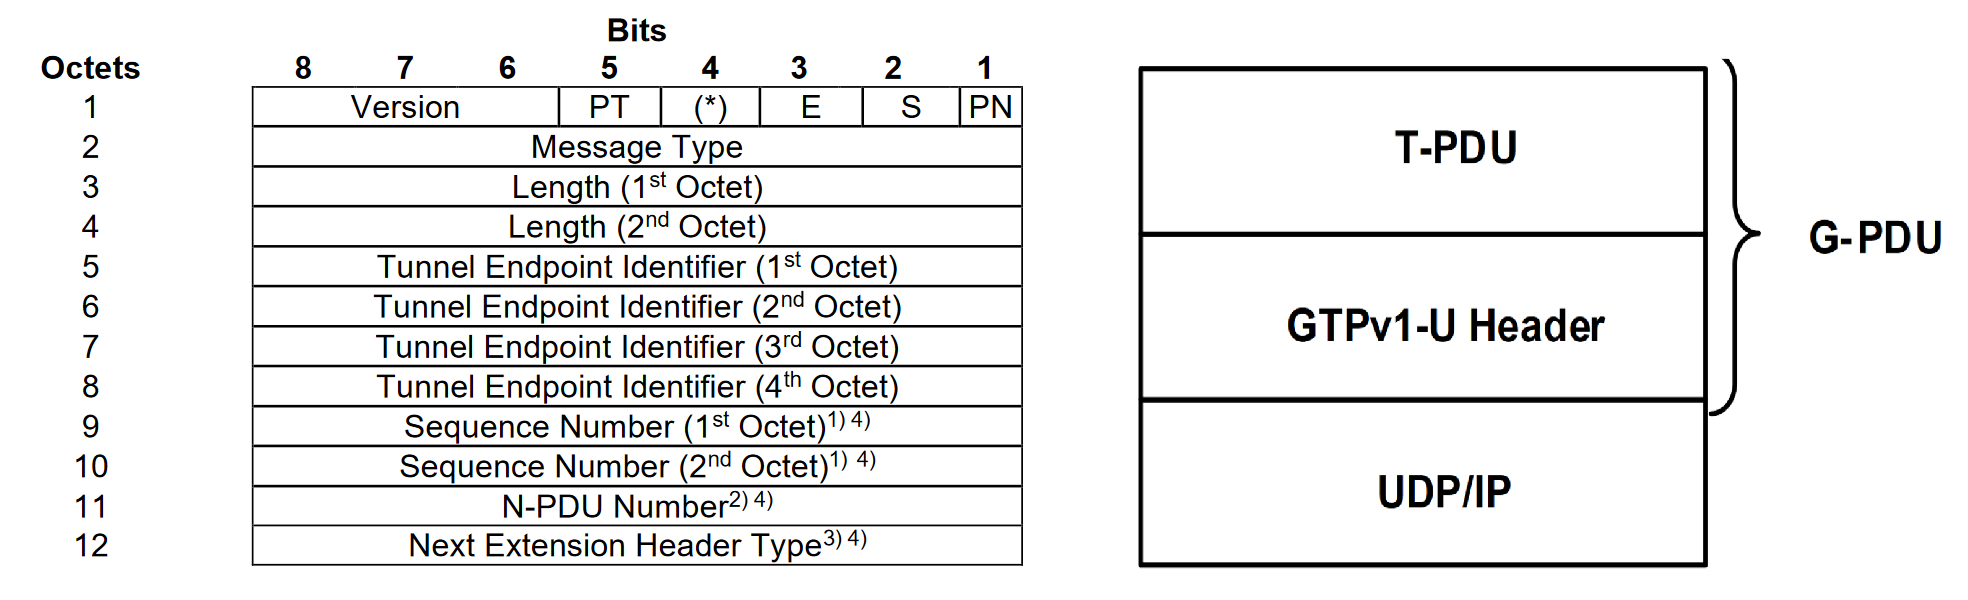
\includegraphics[width=1.0\textwidth]{resources/images/gptu_header_and_gpdu_stack.PNG}
	\caption{3GPP: GPT-U header and G-PDU Protocol Stack built on top of UDP/IP protocol \cite{3gpp_gptu}}
    \label{fig:related_work:gptu_header_and_gpdu_stack}
\end{figure}
